\chapter{Background}

\section{Optimisation}

Optimisation is the process to finding the optimal decision with respect to constraints given a set of possible decisions. The optimal decision is measured by a cost function, that typically determines a numerical value representing how good a decision is. The problem is to either find the optimal decision, either as a minima or maxima using systematic methods. Applications of optimisation occur in many practical situations such as in engineering, manufacturing, science. In engineering applications, accurate modelling of a problem may require discrete decisions and non-linear relationships, resulting in difficulty in finding arbitrary optimal decisions. The wide range of applications of optimisation result in  many fields of optimisation, where in this project we look at MILP.

\begin{figure}[H]
	\begin{center}
		\begin{tikzpicture}
			\node[file](problem) at (0, 2){Problem};
			\node[file](model) at (0, 0){Model};
			\node[file](solution) at (4, 2){Solution};
			\node[file](optimum) at (4, 0){Optimum};
			\draw[arrow](problem) -- node [above] {solve} (solution);
			\draw[arrow](problem) -- node [left, inner sep=10pt] {abstract} (model);
			\draw[arrow](model) -- node [below] {optimise} (optimum);
			\draw[arrow](optimum) -- node [right, inner sep=10pt] {intepret} (solution);
		\end{tikzpicture}
	\end{center}
	\caption{Abstraction of problem solving}
\end{figure}

Real-life problems need to be modelled to be optimised. Problems are formulated using constraints and a cost function. Consider the following linear programming example. A person want to sell some drinks. Each unit of hot chocolate requires 1 litre of milk and 3 bars of chocolate. Each unit of milkshake requires 1 litre of milk and 2 bars of chocolate. The person only has 5 units of milk and 12 bars of chocolate. The person sells a unit of hot chocolate for £6 and a unit of milkshake for £5. What is the best strategy for maximising profit given that all units produced are sold? The problem is abstracted as follows. Let $x$ and $y$ be the number of hot chocolates and milkshakes produced.
\begin{align*}
	\max_{x,y}\ &6x+5y&\text{subject to:}\\
	&x+y\leq 5&\text{milk resource constraint}\\
	&3x+2y\leq 12&\text{chocolate resource constraint}\\
	&x,y\geq 0&\text{non-negative constraints}\\
	&x,y\in\mathbb{N}&\text{whole units only}\\
\end{align*}
The problem is sufficiently small to be solved by inspection, but may also be solved using graphical methods or a simplex algorithm. The optimum is $x^*=2$ and $y^*=3$, which is interpreted as that the best strategy is producing 2 units of hot chocolate and 3 units of milkshake.
\linespace
In non-linear optimisation problems, finding global optimums is not trivial. For gradient-based and local-search algorithms, estimated solutions can return local optimums. This is typically not favoured however for large problems, finding global optimums have non-polynomial complexity for arbitrary dimensional problems. In context of the project, it is unfeasible to compute a complete explanation of optimality in polynomial time.

\subsection{Makeshift Scheduling}

The simplistic definition of makeshift scheduling gives a good foundation for experimenting with argumentation. Makeshift schedules are defined by a $m\in\mathbb{N}$ independent machines and $n\in\mathbb{N}$ independent jobs \cite{sa}. Let $\mathcal{M}=\{1,...,m\}$ be the set of machines and $\mathcal{J}=\{1,...,n\}$ be the set of jobs. Each job $j\in\mathcal{J}$, has an associated processing time $p_j\in\mathbb{R}_{\geq 0}$. All processing times are collectively denoted by a vector $\mathbf{p}$. A machine can only execute at most one job at any time. For a feasible schedule, each job is assigned to a machine non-preemptively. For some $i\in\mathcal{M}$, let $C_i$ be the completion time of the $i^\text{th}$ machine. Let $C_{\max}$ be the total completion time. Let $\mathbf{x}\in\{0,1\}^{m\times n}$ be the assignment matrix that allocates jobs to machines. Formally, makeshift schedules are modelled as an optimisation problem:
\begin{align*}
	\min_{C_{\max},\mathbf{C},\mathbf{x}}\ &C_{\max}&\text{ subject to:}\\
	\forall i\in\mathcal{M}.\ &C_{\max}\geq C_i\\
	\forall i\in\mathcal{M}.\ &C_i=\sum_{j\in\mathcal{J}}x_{i,j}\cdot p_j\\
	\forall j\in\mathcal{J}.\ &\sum_{j\in\mathcal{J}}x_{i,j}=1\\
	\forall i\in\mathcal{M},\ \forall j\in\mathcal{J}.\ &x_{i,j}\in\{0,1\}
\end{align*}

\begin{definition}
	A schedule $S$ is defined by its assignment matrix $\mathbf{x}$ such that $S=\mathbf{x}$. $S$ will be used to reference a high-level representation of $\mathbf{x}$ but does not specify its formal representation unlike $\mathbf{x}$, which will be used in linear programming and algorithms with its precise definition.
\end{definition}

\begin{definition}
	A schedule $S$ is optimal iff $S$ achieves the minimal total completion time.
\end{definition}


\begin{definition}
	A machine $i\in\mathcal{M}$ is critical iff $C_i=C_{max}$.
\end{definition}

\begin{definition}
	A job $j\in\mathcal{J}$ is critical iff $j$ is allocated to a critical machine $i\in\mathcal{M}$ and $x_{i,j}=1$.
\end{definition}

\begin{definition}
	A schedule satisfies the single exchange property (SEP) iff for any critical machine and any machine $i,i'\in\mathcal{M}$ and for all critical jobs $j\in\mathcal{J}$, $C_i-C_{i'}\leq p_j$
\end{definition}

\begin{definition}
	A schedule satisfies the pairwise exchange property (PEP) iff for any critical job and any job $j,j'\in\mathcal{J}$, if $p_j>p_{j'}$, then $C_i+p_{j'}\leq C_{i'}+p_j$.
\end{definition}

\begin{definition}
	A schedule $S$ is efficient iff $S$ satisfies SEP and PEP.
\end{definition}

\begin{theorem}
	Schedule efficiency is a necessary condition for optimality.
\end{theorem}

Makeshift schedules are often represented using cascade charts. The charts shows graphically the difference in total completion time of schedules where the problem has the parameters $m=4$ and $n=13$.

\begin{figure}[H]
	\begin{center}
		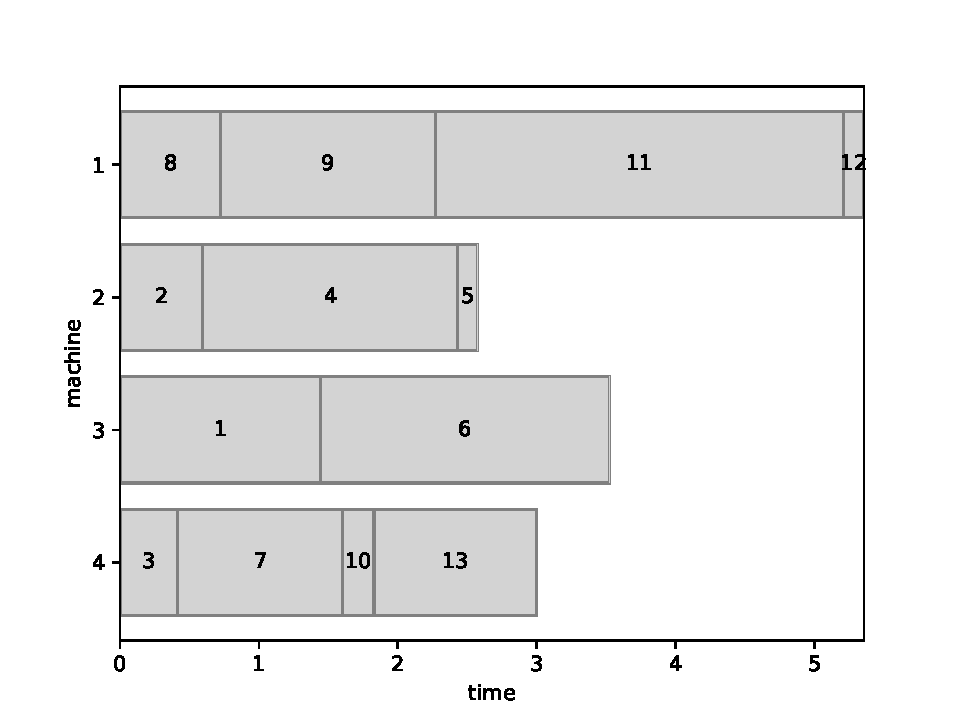
\includegraphics[width=.6\linewidth]{figures/makeshift_inefficient.pdf}
	\end{center}
	\caption{An inefficent schedule}
\end{figure}

\begin{figure}[H]
	\begin{center}
		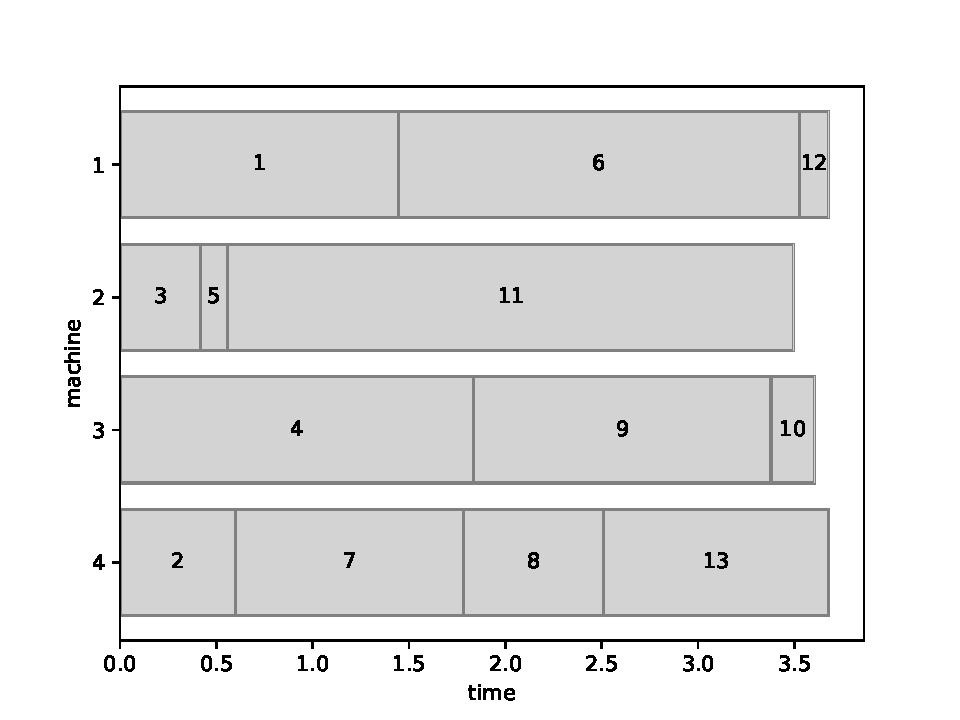
\includegraphics[width=.6\linewidth]{figures/makeshift_efficient.pdf}	
	\end{center}
	\caption{An efficient schedule}
\end{figure}

\subsection{User Fixed Decisions}

To accommodate practical applications of makeshift schedules, user positive and negative fixed decisions are introduced as an extension to makeshift problems. In a hospital setting, positive fixed decisions capture patients exclusively allocated to a nurse while negative fixed decisions capture unavailable or incompatible nurses and patients \cite{aes}. Let $D^-,D^+\subseteq\mathcal{M}\times\mathcal{J}$ be the negative and positive fixed decisions respectively. Let $D$ be the fixed decisions such that $D=(D^-,D^+)$.

\begin{definition}
	A schedule $S$ satisfies $D$ iff $\forall(i,j)\in D^-.\ x_{i,j}=0$ and $\forall \pair{i}{j}\in D^+.\ x_{i,j}=1$.
\end{definition}

\begin{definition}
	A fixed decision $D$ is satisfiable iff there exists a schedule $S$ such that $S$ satisfies $D$. 
\end{definition}

\begin{theorem}
	A fixed decision $D$ is satisfiable iff if the following necessary and sufficient conditions hold:
	\begin{itemize}
		\item$D^+$ and $D^-$ are disjoint.
		\item$\forall\pair{i}{j},\pair{i'}{j'}\in D^+.\ i=i'\lor j\neq j'$
		\item$\forall j\in\mathcal{J}.\ \exists i\in\mathcal{M}.\ \pair{i}{j}\not\in D^-$
	\end{itemize}
\end{theorem}

The relaxed definition of $D$ allows $D$ to be unsatisfiable, which is not permitted in previous work \cite{aes}. This relaxation accommodates for poorly-formulated user problems, allowing explanations over validation of user input, which is more useful to users in a practical setting.

\subsection{Interval Scheduling}

Interval scheduling is a natural extension to makeshift scheduling. Makeshift scheduling has freedom in determining the starting times of its jobs. In practice, rearranging critical jobs may effect the feasibility of a schedule. Interval scheduling is a widely researched area, with many literature proposing algorithms for variants of interval scheduling \cite{is}.
\linespace
Interval scheduling is defined over $m\in\mathbb{N}$ and $n\in\mathbb{N}$ jobs where they are collectively denoted by the sets $\mathcal{M}$ and $\mathcal{J}$ such that $\mathcal{M}=\{1,...,m\}$ and $\mathcal{J}=\{1,...,n\}$ respectively. Each job $j\in\mathcal{J}$ must be allocated a machine $i\in\mathcal{M}$ preemptively. In addition, each job must be allocated between the interval $[s_j,f_j)$ such that $s_j<f_j$ where $s_j,f_j\in\mathbb{R}_{\geq 0}$ without loss of generality. Finally, each job is associated with a processing time $p_j\in\mathbb{R}_{\geq 0}$. No jobs are allowed to overlap. Note that $p_j>f_j-s_j$ is possible, meaning that interval schedules can be constructed to be infeasible.

\section{Argumentation}

Argumentation is a method to understand and evaluate reasons for and against potential conclusions. Argumentation is useful in resolving conflicts, clarifying incomplete information and most importantly, with respect to this project, explanations. The precise definition of an argument varies on the literature, however it is commonly agreed that arguments can attack or support other arguments. For an argument $\alpha$ to attack an argument $\beta$, $\alpha$ may critically challenge $\beta$ such that acceptability of $\beta$ is doubted \cite{at}. This may be to question one of $\beta$'s premises, by proposing a counter-example. For example, consider an scenario whether to sleep. Let $\alpha$ be ``I want to sleep", $\beta$ be ``I have work to do" and $\gamma$ be ``I can work tomorrow". Using human intuition, we can derive that $\gamma$ attacks $\beta$ and $\beta$ attacks $\alpha$. This is represented graphically below.

\begin{center}
	\begin{tikzpicture}
		\node[node](gamma) at (0, 0){$\gamma$};
		\node[node](beta) at (2, 0){$\beta$};
		\node[node](alpha) at (4, 0){$\alpha$};
		\draw[arrow](gamma) -- (beta);
		\draw[arrow](beta) -- (alpha);
	\end{tikzpicture}
\end{center}

If we conclude $\alpha$ to be acceptable, then we must not accept $\beta$. Accepting two arguments with conflicts can be interpreted as a contradiction or hypocritical. Hence, argumentation theory have measures of acceptable extensions, to decide whether some set of arguments are acceptable in some notion, with respect to different intuitions. This motivates to use abstract argumentation frameworks.\linespace
Note that this example uses implicit background knowledge, also known as enthymemes. In this scenario, one cannot sleep and work at the same time. To our advantage, argumentation is applied to well-defined scheduling problems, so enthymemes are inapplicable in this project.

\subsection{Abstract Argumentation Frameworks}

An abstract argumentation framework (AAF) models the relation of attacks between arguments \cite{aa}. Formally, an AAF is a directed graph $(Args,\rightsquigarrow)$ where $Args$ is the set of arguments and $\rightsquigarrow$ is a binary relation over $Args$. For $a,b\in Args$, $a$ attacks $b$ iff $a\rightsquigarrow b$. Attacks are extended over sets of arguments, where $A\subseteq Args\rightsquigarrow b\in Args$ iff $\exists a\in A.\ a\rightsquigarrow b$. An extension $E$ is a subset of $Args$.

\begin{definition}
	An extension $E$ is conflict-free iff $\forall a,b\in E.\ a\not\rightsquigarrow\ b$.
\end{definition}

\begin{definition}
	An extension $E$ is stable iff $E$ is conflict-free and
	
	$\forall a\in Args\backslash E.\ E\rightsquigarrow a$
\end{definition}

\begin{figure}[H]
	\begin{center}
		\begin{tikzpicture}
		\node[node](gamma) at (0, 0){$\gamma$};
		\node[node](beta) at (2, 0){$\beta$};
		\node[node](alpha) at (4, 0){$\alpha$};
		\node[node](delta) at (2, 2){$\delta$};
		\node[node](epsilon) at (0, 2){$\varepsilon$};
		\draw[arrow](beta) -- (alpha);
		\draw[arrow](beta) -- (gamma);
		\draw[arrow](beta) -- (delta);
		\draw[arrow](delta) -- (beta);
		\draw[arrow](delta) to [loop](delta);
		\draw[arrow](epsilon) -- (delta);
		\end{tikzpicture}
	\end{center}
	\caption{An AAF represented graphically}
\end{figure}

Consider the following example where $Args=\{\alpha,\beta,\gamma,\delta,\varepsilon\}$ and $	\rightsquigarrow=\{
\pair{\beta}{\alpha},\\
\pair{\beta}{\gamma},
\pair{\beta}{\delta},
\pair{\delta}{\beta},
\pair{\delta}{\delta},
\pair{\varepsilon}{\delta}
\}$ as illustrated above. Then the following statements hold:
\begin{itemize}
	\item $\varepsilon\rightsquigarrow\delta$.
	\item $\{\delta,\varepsilon\}\rightsquigarrow\beta$.
	\item $\{\alpha,\gamma\}$ is conflict-free but not stable.
	\item $\{\delta\}$ is not conflict-free and not stable.
	\item $\{\beta,\varepsilon\}$ is conflict-free and stable.
\end{itemize}

\begin{definition}
	An extension $E$ is admissible iff $E$ is conflict-free and $E$ attacks every argument attacking $E$.
\end{definition}

\begin{definition}
	An extension $E$ defends an argument $\alpha$ iff for all every argument attacking $\alpha$, $E$ attacks such attacking argument 
\end{definition}

\begin{definition}
	An extension $E$ is complete iff $E$ is admissible and $E$ contains all arguments $E$ defends.
\end{definition}

\begin{definition}
	An extension $E$ is preferred iff $E$ is maximally admissible with respect to $\subseteq$.
\end{definition}

\section{Explanations}

Explanation generation problems are a class of explainable planning problems. Many generation tasks appeal to either minimality or simplicity \cite{pe}. Explanations may occur over observations. For example, a sequence of states may lead to an error, an explanation can guide an agent to avoid such error. However, trustworthy and theoretical well-understood algorithms are difficult to explain to non-technical users \cite{ep}. The paper highlights concepts to explain given an optimisation context:
\begin{itemize}
	\item Why did the optimiser do that?
	\item Why did the optimiser not do this?
	\item Why does this proposal result to more optimal result?
	\item Why can't this decision be taken?
	\item Why do I need to re-plan at this point?
	\item Will a better result be produced if given $n$ more hours?
\end{itemize}

Arguably, understanding cannot be captured with a few questions. Future question include the negation, where their answers are not natively their negation.

\section{Existing Tools}

We will look at two scheduling software, Setmore and LEKIN, in terms of explainable planning. We will not look existing tools using argumentation because of relevancy, we use argumentation as a means of explanation in an intermediate process.

\subsection{Setmore}

\begin{figure}[H]
	\begin{center}
		
\includegraphics[scale=0.4]{figures/setmore_gui.png}
	\end{center}
	\caption{Setmore interactive interface \cite{setmore}}
\end{figure}

Setmore is a commercial online application that records appointments, schedules and employees. The application is designed for small business such as in healthcare \cite{setmore}, where managers can organise appointments on a calender. Makeshift schedules are formulae where employees are machines and appointments are jobs. The intuitive interface enables users to quickly glance at appointments and their times, it is graphically clear when two appointments overlap. However, under the condition that one employee is able to attend at most one appointment, the user is presented with an error message. Messages also occur when resources are fully-booked or unavailable. Scheduling error messages alert the user during data input, which may prove problematic when a user wishes to input a large number of appointments. Appointments cannot be over-allocated because each appointment has at most assignment one by interface restrictions.

\begin{figure}[H]
	\begin{center}
		
\includegraphics[scale=0.6]{figures/setmore_overallocated.png}
	\end{center}
	\caption{Overlapping appointment allocation error message}
\end{figure}

\begin{figure}[H]
	\begin{center}
		
\includegraphics[scale=0.6]{figures/setmore_no_service.png}
	\end{center}
	\caption{Data input of an appointment where there are no possible services, or possible assignments}
\end{figure}

We will assess the application under its free-trail, which may limit its explanative functionality. A key observation is that there is no emphasis on the concept of an optimal schedule. Because the tool is designed for small businesses and optimality is not well-defined for arbitrary businesses, the user can graphically inspect and improve a schedule with respect to the user's notion of optimality. Modification of an existing schedule is well-facilitated within its interface, where appointments can be moved or swapped between employees. Explanations for unfeasible schedules are limited to data input verification and validation error messages.

\subsection{LEKIN}

\begin{figure}[H]
	\begin{center}
		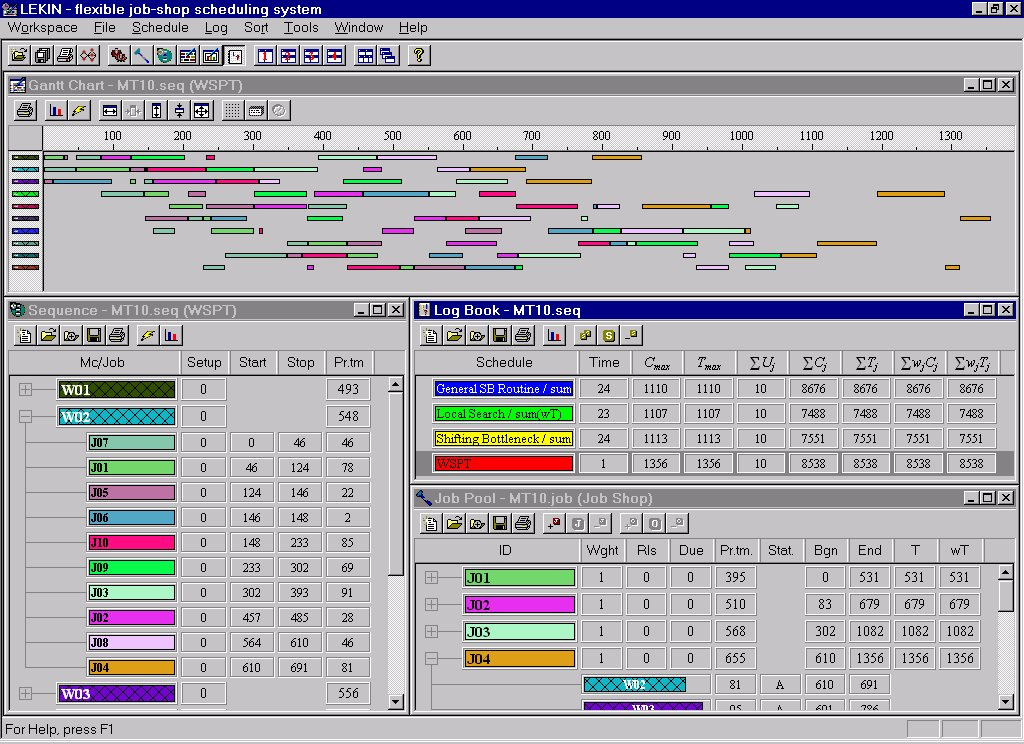
\includegraphics{figures/lekin_gui.jpg}
	\end{center}
	\caption{LEKIN interactive interface \cite{lekin}}
\end{figure}

LEKIN is a academic-oriented scheduling application to teach students scheduling theory and its applications, developed at the Stem School of Business, NYU \cite{lekin}. The application features numerous optimisation algorithms specialised for scheduling and draws inspiration from academic for rules and heuristics \cite{sta}. The tool supports single machines, parallel machines and flexible job shop settings.

\begin{figure}[H]
	\begin{center}
		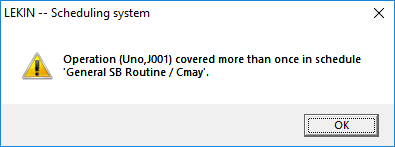
\includegraphics[scale=0.8]{figures/lekin_overallocated.png}
	\end{center}
	\caption{Over-allocation of a job to multiple machines}
\end{figure}

\begin{figure}[H]
	\begin{center}
		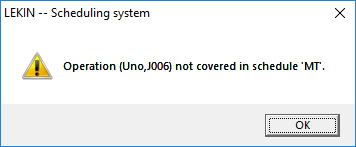
\includegraphics[scale=0.8]{figures/lekin_unallocated.png}
	\end{center}
	\caption{A job is not allocated to any machine}
\end{figure}

The application validates a schedule's feasibility at data input. Infeasible schedule results in error messages. The application computes optimal schedules, but has no functionality to verify its optimality. While our approach is to weaken optimality with efficiency, LEKIN takes the approach to compute common scheduling performance metrics such as makeshift completion time, tardiness and weighted metrics over machines. The advantage is that these metrics can be easily and quickly be computed and are intuitive to non-technical users given some background reading. However, these metrics are global across all machines, and give no indication to improving schedules. Non-technical users may run one of the provided optimisers to improve metrics, but no explanation is offered between the assignments of the pre-optimised and the post-optimised schedules.

\begin{figure}[H]
	\begin{center}
		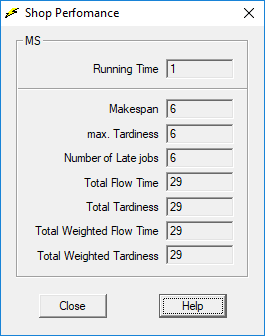
\includegraphics[scale=0.8]{figures/lekin_metric.png}
	\end{center}
	\caption{Performance metrics of an schedule}
\end{figure}

\subsection{Comparison}

It is clear that both application offers limited explanations, explicitly by error messages and implicitly by cascade charts. However, both methods require human intuition, which is unfeasible for large schedules. Therefore, for effective knowledge transfer, localised text explanations and cascade charts help users to focus on key machines and jobs.